%# -*- coding: utf-8-unix -*-
%%==================================================
%%==================================================

\chapter{绪论}
% \label{chap:intro}

\section{研究背景和意义}
一般在传统的医疗诊断和治疗方案决策的过程中,医生一般先要求病人进行详细全面的查体。这里查体的结果被视作一系列针对病人的理化指标。根据这些理化指标,医生再结合病人的临床病史,病人当前的状态,医生的专业知识与临床经验以及制定好的相关治疗规范或治疗手册对病人的疾病状态做进一步评估并给出合理的治疗方案。

大多数情况下病人的状态都可以用医学或者生物学的术语作准确地描述,医生也可以根据自己的知识作出较为准确的判断。对于许多典型的病例,医疗手册中可以找出符合的最优治疗方案,如果这个过程能够自动化,便可以极大程度上提升医生诊断的工作效率。但事实上很多病例并没有完美匹配医疗手册中的规则,这种情况下对病例情况的判断很大程度上依赖于医生自身的水平,具有较大的主观因素:对于一个刚刚完成职业规范化培训的医生,他的临床经验可能比较欠缺;而对于一个从医数十载的专家,他的技术可能极为精湛。考虑到医生的水平参差不齐,以及医生思考问题的角度可能不尽相同,不同的医生对同一个病例可能持有不同的态度,即每个医生心中对同一个病例的最佳治疗方案可能大相径庭。

与此同时,现代医学飞速发展,医学中各个分支领域的划分越来越细,各个方向的知识越来越深入,一个专攻某个领域的专家由于知识面相对地狭窄,因而不能凭借一己之力同时兼顾病患自身的其他方面的因素,这势必造成对病患的诊断有一定的片面性。这种情况下,多学科综合治疗(Mulity-Disciplinary Treatment,简称MDT)的概念\cite{Taylorc951}应运而生。多学科治疗是一种组织多学科协作诊治病情的形式,即由来自医院放射科、病理科、检验科、心电图、普外科等相关科室,甚至包括医联体内其他外部专家组成工作组,针对某一疾病,通过会诊方式提出适合患者的最佳治疗方案并多学科联合执行。主要针对肿瘤、疑难复杂疾病、多系统多器官疾病等。MDT综合了不同医疗领域专家的共同智慧从而保证高质量的诊治建议和最佳的治疗计划,避免过度诊疗和误诊误治,使病人受益最大化。

随着计算机科学与软件工程的发展,为了支持多学科综合治疗会议的展开,决策支持系统(Decision Support system,简称DSS)作为一个高效的工具,曾一度被不同学科的科研工作者所重视\cite{Filip2017}。智能决策系统的出现,使得高效的,大规模的多学科治疗案例得以实施。该系统的意义在于整合医疗资源,维护医疗决策过程,并总结相关知识反馈给医生,辅助医生来做判断与决策。以多学科治疗为目的的决策支持系统简称MDTDSS。智能决策系统有两大方向,分别是基于规则的系统和基于历史案例的系统。

基于规则的系统主要利用到了知识表示方法中将规则符号化的方法\cite{Ligêza2006}。该方法将规则抽象化成逻辑公式,将病人的各种指标作为输入,推导出正确的结果。这里的规则一般来源于许多医疗机构发布并使用的权威医学指南,例如国家综合癌症治疗网络(National Comprehensive Cancer Network,简称NCCN)\cite{Mohler2010The}。但是,这些指南建议的治疗方案通常是粗略的,例如可以根据病人的情况推导出该病人需要化疗却无法推导出需要哪种类型的化疗。另外,对于有些特殊的病例,并没有匹配治疗指南中的某个规则,则如果把这样的病例作为输入,系统根本无法得到一个结果。

另一个方向是基于历史病例数据的决策支持系统。基于历史病例的决策也称作基于案例的推理,对它最早的研究发生在二十世纪七十年代后期\cite{Schank1988SCRIPTS,Schank1982Dynamic}。这样的系统维护了一个供多学科团队讨论的平台,在该平台上,多学科团队的诸位专家对同一个病例多次发表意见。这些意见最终由专人进行汇总,采用投票的方式决定该病人的最终治疗方案。图\ref{fig:ch1-1}展示了某决策支持系统的多学科团队讨论模块。整个讨论过程分为三个步骤:初次投票环节,决议投票环节以及决策环节。\textbf{在初次投票环节,}医生根据病人的情况以及自己的专业知识与经验,互相独立地为病人选择一个合理的化疗方案。在该环节,多学科团队中的各个医生无法知道其他医生的意见\textbf{在决议投票环节,}医生参考其他医生对该病例的意见,可以对自己在第一轮投票的结果进行修改,或者继续坚持自己在前一轮做出的决定。\textbf{在决策环节,}投票负责人汇总决议投票的结果,以少数服从多数的方式,决定病人的最佳化疗方案。如图\ref{fig:ch1-1}所示的案例中,在决议投票之后,共有11位医生为该病人选择了EC-T方案,数量最多。因此该病人最终的化疗方案被制定为EC-T。这样一个讨论过程中,可以挖掘的知识主要有以下三个方面:
\begin{enumerate}
  \item 每位医生在初次投票中对病例情况做出的独立判断
  \item 每位医生在决议投票中对病例情况的判断发生变化的情况
  \item 该病人对应的最佳治疗方案
\end{enumerate}
这样的基于历史病例数据的决策支持系统,通过维护一个又一个对病例的讨论过程,并将讨论数据做持久化处理,可以构造出一个完整的关于疾病治疗方案的知识库。近年来,人工智能技术越来越多的得到人们的重视,人工智能与机器学习的相关算法已经深入到包括金融,生活,出行等诸多领域。将人工智能算法应用于病例知识库,对上述三种知识加以总结与分析,可以对病人的最佳治疗方案进行推荐,并把推荐结果反馈给医生,帮助医生更好的做出判断。这对于整合医疗资源与医学知识,补充医生知识与经验的缺陷以及实现精准医疗、高效医疗有重要的意义。

此外,针对基于历史病例数据的决策支持系统的本质是将待推荐病例与病例数据库中的已有知识相对比并作出相应的判断。这其中中所使用的相关推荐算法,一旦效果显著,很可能被大规模推广与使用。这样的系统可能具有较高的QPS(Queries-per-second,每秒查询率)与DAU(Daily Active User,日活跃用户数量)并且拥有相当大规模的病例数据库。同一时刻可能有多位用户并发地访问该系统,并希望系统针对某个病人,根据病理数据库中的知识获得其推荐的治疗方案。巨大的数据量与有限的算力资源之间的矛盾必然将导致推荐的时延显著增加。如何优化推荐算法以减小问题的规模,如何折中算法的复杂度与推荐结果的准确率,也是本文关注的另一个重点。

综上,本文以医疗方案的基本推荐方法为出发点,先后介绍基于规则和基于历史数据的医疗方案推荐方法,并提出了相应的优化方法;之后,本文以专家的投票数据为基础,对历史病例数据做进一步挖掘以提升推荐的性能;然后,考虑到这样的方法落地并被大规模使用之后,推荐的时延和算法的问题规模可能带来的瓶颈问题,本文提出了折中相应算法复杂度与推荐准确率的方法。在最后,本文将详细介绍相应的系统实现。
\begin{figure}[!htp]
  \centering
  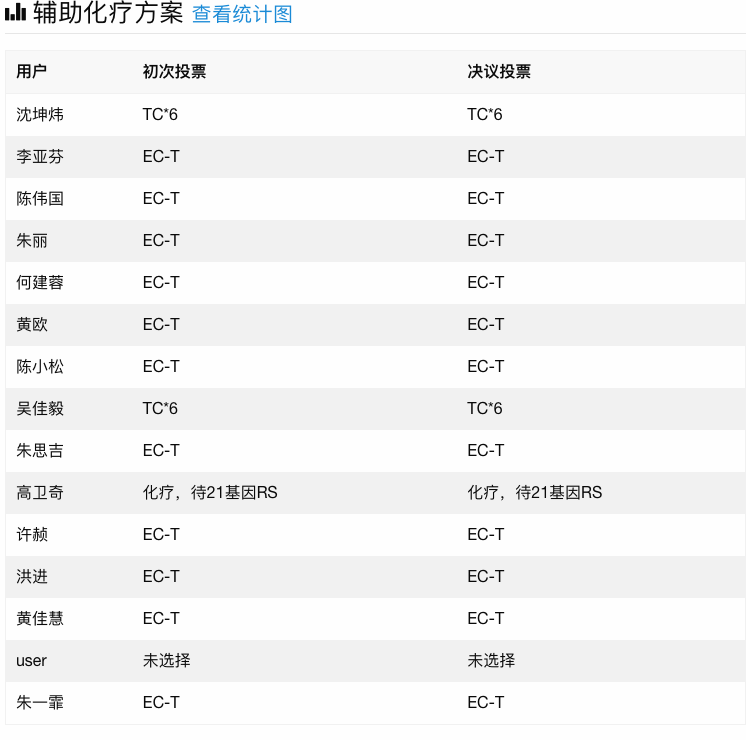
\includegraphics[width=10cm,height=12cm]{figure/ch1-fig1.png}
  \bicaption[某决策支持系统的多学科团队讨论结果]
    {某决策支持系统的多学科团队讨论结果}
    {the result of the discussion part of one MADTDSS}
  \label{fig:ch1-1}
\end{figure}

\section{国内外研究现状}

近年来,将计算机科学方法应用于治疗方案推荐一度成为科研人员的研究热点。其中提出的医疗方案推荐方法大致可以分为两个方向,分别是基于规则的推荐方法以及基于历史数据的推荐方法。本节将先后探讨基于规则的医疗推荐方法的研究现状,基于历史数据的医疗推荐方法的研究现状以及决策支持系统的研究现状。

\subsection{基于规则的医疗推荐方法}

处理诸如心力衰竭,糖尿病和慢性阻塞性肺疾病,癌症等慢性疾病是医疗中的主要问题。医学指南一般是指由一些权威医疗机构的医疗委员会的专家成员制定的,所有医师都应该遵循的,主要用于管理慢性疾病的标准方法。这些准则通常由一系列
根据患者信息提出建议的复杂规则组成。一般医疗指南都具有较长的篇幅与复杂的逻辑。比如针对慢性心力衰竭的医疗指南有80页。由于其复杂性,通常这些准则要么被忽略,要么根本不遵守,这可能导致不良的医疗实践。为了解决这一问题,在2016年,Chen Zhuo等人在文献\parencite{Chen2016A}之中描述了一种用于CHF管理的医生咨询系统,该系统使用答案集编程为CHF的整个临床实践指南进行编码。所使用的方法基于开发推理模板(即知识图谱),并使用这些模式将CHF的临床指南系统编码为ASP规则。知识图谱的使用极大地简化了系统的开发。当患者的状态和各种理化指标给定后,即使信息不完整有缺失,系统也可以像医生一样给出治疗建议。该系统的成功实践有两个明显的意义:1)该系统的成功实践表明高度复杂的准则可以成功地编码为ASP规则,2)该系统开发出一系列知识模式,这些模式有助于对以自然语言表达的知识进行编码,并可以用于其他应用领域。

对慢性疾病进行有效的临床管理有时还需要一系列治疗,每种治疗均应适应个体反应,因此需要在个人临床护理的整个过程中做出多种治疗决定。在2011年,Daniel Almirall等人提出了自适应治疗策略(adaptive treatment strategies,简称ATS)\cite{Daniel2012Designing}。ATS使得这样一系列的治疗规则化。ATS通过“关键规则”来实现个性化治疗。“关键规则”主要定义了是否,如何,以及何时改变治疗的方式与强度。关键决策的例子包括最初提供哪种治疗,等待初始治疗多长时间,如何确定初始治疗是否有效,以及如果初始治疗可以提供下一个治疗治疗有效或无效。每个关键决策的治疗方法可能包括药物,行为治疗干预,或两者结合。ATS将患者的治疗状况最为输入,将推荐的该阶段的治疗方法作为输出。为了将ATS各个阶段的最优化输出组合成为一套最优的治疗方案,文献\parencite{Daniel2012Designing}又提出了连续性多次分配实验(Sequential multiple assignment randomized trials,简称SMART)。SMART的关键特征是,它允许研究者通过使用随机数据,以原则性方式评估治疗的时机,顺序和对ATS的决策结果做出适应性选择。2016年,为了评估使用ATS和SMART对青少年抑郁症治疗的可行性,Gunlicks-Stoessel等人使用4条ATS展开了临床试验\cite{Gunlicks2017A};并对32名青少年进行了为期16周的连续性多次分配实验(SMART),初步研究的结果对全尺寸SMART提出了更多的研究问题。


\subsection{基于历史数据的医疗推荐方法}
针对基于历史病例数据的决策支持系统的本质是将待推荐病例与病例数据库中的已有知识相对比并作出相应的判断。由于复杂的疾病和药物依赖性以及药物不良相互作用的潜在风险,长期以来,对具有多种并发症的患者进行治疗一直是一个难题。不同于基于难以使用的高度复杂的规则的医疗推荐方法与基于简单统计模型的方法,Yutao Zhang等人在2017年提出了LEAP算法\cite{Zhang2017LEAP},该算法将医疗推荐分解为一系列决策过程以自动确定合适的药物数量。在文献\parencite{Zhang2017LEAP}中,循环解码器用于捕获标签实例映射的标签相关性,强化学习的相关方法用于对模型参数进行相关微调,以确保结果的完整性与准确性。文献\parencite{Zhang2017LEAP}创新性地提出外部临床知识纳入强化奖励的设计中,以有效防止产生不利的药物组合。在真实世界的电子健康记录数据集上进行了定量实验和定性案例研究表明,LEAP算法有效地消除了推荐治疗组中99.8%的不良药物相互作用。

在文献\parencite{Zhang2017iDoctor}中,介绍了一种名为iDoctor的新型医疗保健推荐系统,该系统基于混合矩阵分解方法。 iDoctor在以下方面与先前的工作有所不同:(1)用户评论的情感偏移可以通过情感分析来揭示,并可以用来修改原始用户评分; (2)通过Latent Dirichlet Allocation提取用户偏好和医生特征,并将其合并到常规矩阵分解中。 献\parencite{Zhang2017iDoctor}使用实际数据集将iDoctor与以前的医疗保健推荐方法进行了比较。 实验结果表明,iDoctor提供了更高的预测评分,并显着提高了医疗保健推荐的准确性。

文献\parencite{Thong2015HIFCF}考虑了将直觉模糊集(IFS)和推荐系统(RS)集成到所提出的方法中,并提出了一种新颖的直觉模糊推荐系统(IFRS)。与仅在传统模糊集或推荐系统上构建的相关方法相比,IFRS的预测精度更高。在观察到通过整合模糊聚类方法指定的聚类患者的可能性信息可以增强IFRS相似度计算的基础上,文献\parencite{Thong2015HIFCF}还提出了图像模糊聚类与直觉模糊之间的一种新型混合模型:HIFCF(混合直觉模糊协作过滤)。实验结果表明,HIFCF比IFCF具有更好的准确性。

2014年Pradhan等人\cite{Pradhan2014Improving}引入了一种创新的基于信任的信息模型来评估那些牙科相关评论以及调查中患者的主观因素。该模型评估了4个信任成分:上下文,关系,声誉和性格分析。使用此模型以及从社交网络中提取的信息对牙医和患者的关系进行剖析。使用从在线牙科评论获得的主观素质对牙医进行剖析,并使用从580名参与者中收集的调查结果等主观信息对患者进行剖析,例如个体对牙医的恐惧程度和人格特质。研究的结果可用于定义一套规则,以改善牙科保健推荐系统中患者和牙医之间的匹配程度。


\subsection{决策支持系统}
对决策支持系统(Decision Support system,简称DSS)的研究最早可以追溯到10年以前\cite{Filip2017}。本节将近十年以来各个领域的科研工作者对决策支持系统所做的研究进行总结,将其大致分为以下五种类型:

\begin{itemize}
\item \textbf{基于模型的DSS。}

基于模型的DSS以一个简单的数学模型为系统的核心。这种系统的着眼点主要放在如何访问与操作模型上。基于模型的DSS一般根据用户输入的数据以及用户对系统的相关配置为用户的决策提供帮助,但是一般而言,系统的数据量不大,不需要规模庞大的数据库。
\item \textbf{基于通信的DSS。}

基于通信的DSS利用诸如RPC协议\cite{Srinivasan1995RPC}等网络通信技术来促进系统中不同服务之间的协作以提升系统的性能。这样的系统以网络与通信技术为核心。上世纪后期,一部分工程师设计了群体DSS以支持群体性质的决策任务\cite{Turoff1982Computer}。之后又出现了一系列基于通信技术的DSS诸如Arizona大学所研发的Group Systems系统,Minnesota大学研发的SAMM系统等。一般来说基于通信的DSS在应用层使用到的主要技术主要包括公告板,音视频在线会议等。近几年由于网络技术发展迅猛,基于通信的DSS的发展速度也出现了显著的提升。

\item \textbf{基于数据的DSS。}

基于数据的DSS的底层是一个由内部以及外部数据,时序或者非时序的数据构成的数据库或者数据仓库\cite{Stumme2000Conceptual}。这样的系统既可以仅仅由简单的文件系统构成,也可以为用户提供一些用于查询或者检索的接口。也可以将这样的系统服务化,同时加入数据分析服务,使得系统更加复杂的同时,帮助用户做相应的分析,通过数据库中海量的数据作进一步的数据挖掘,并为用户提供更智能,更加多元的服务。
\item \textbf{基于文档的DSS。}

基于文档的DSS的核心在于利用先进的计算机存储与搜索引擎技术对文件进行管理。这里的文档可能包括音频,视频,图片,文本文件等。除开底层存储的数据更加多元化意外,基于文档的DSS也类似地为用户提供相应的管理接口。

\item \textbf{基于知识的DSS。}
基于知识的DSS两个典型的例子就是近来颇为热门的智能问答系统与专家系统\cite{Buchanan1984Rule,Gonzalez1985The}。两个典型的基于知识的DSS包括\parencite[]{Buchanan1984Rule,Gonzalez1985The}。它主要包括帮助领域内专家解决问题以及理解领域内专业知识问题的能力。

\end{itemize}

\section{本文主要内容与结构安排}

\subsection{本文的主要内容}
本文的工作紧密围绕医疗方案的推荐方法而展开,大致内容包括医疗数据的特征工程;基于案例的医疗方案推荐方法;基于历史病例数据的医疗方案推荐方法;基于专家意见与历史数据的医疗方案推荐方法;基于数据的推荐方法的规模问题讨论;一个具有医疗方案的推荐模块的多学科团队智能决策支持系统的具体实现。本文大主要内容具体地可以描述为以下几个方面:

\begin{enumerate}
  \item 研究所基于的数据来源,以及数据格式。数据主要分为结构化与非结构化数据两大类,本文讨论了研究利用的数据如何从庞大的数据中找出需要的几个典型的几个维度。如何将数据格式化,并转化成特征向量。
  \item 在如何根据特征向量依据规则对病人做医疗方案的推荐方面,本文介绍了几个典型的规则。同时介绍了基于规则作出决策的方法,然后通过实验对基于规则的医疗方案推荐方法进行了分析。
  \item 本文深入探讨了基于历史数据的医疗方案推荐方法。首先,本文介绍了特征向量的构成以及特征的进一步筛选,以及筛选的原则。之后本文采用knn算法对历史数据进行挖掘,并实施了相关的实验以论证方法的有效性。在这部分的最后,深入地研究了如何对基本的knn算法进行优化,这种优化主要体现在对特征向量中不同的属性的权重上。本文提出了多种不同权重的训练方案,最大限度的对模型进行了优化。
  \item 针对通过knn算法找出相似历史数据后,如何根据它们做决策,以及历史数据标签本身的不确定性这两个比较核心的问题。本文以Dempster Shafer的证据融合理论为核心进行建模,对每个历史病例专家的投票信息进行量化分析,将不确定度融合到最终的决策中。同时依赖于此模型,使用神经网络对特征向量中的属性的权重进行表示学习,使得模型在推荐的效果上得到了进一步的优化。
  \item 本文详细对前面的算法的规模问题进行了详细的讨论,并对算法的时间复杂度做了充分的分析。考虑到本文涉及的方法被应用于系统之后可能带来较高的计算时延以影响用户体验,本文创新性地使用边界树算法来对基于历史标签不确定性的算法进行在线化处理。这种做法实际是对计算速度和准确率的一种折中。实验结果表明,基于边界树的优化算法可以在几乎不损失推荐准确度的情况下极高程度的简化计算的规模。
  \item 在最后,本文介绍了一个拥有医疗方案推荐功能的多学科团队智能决策辅助支持系统的系统架构以及具体实现;详细地介绍了其中使用到的关键技术并展示了一些UI界面;最后介绍了系统比较特色的几个功能,比如病例复杂程度展示等。
\end{enumerate}

\subsection{本文的结构安排}

第一章是绪论,这一章中主要介绍了研究背景及本文所涉及方向的国内外研究现状,具体分别包括基于规则的推荐方法,基于历史数据的推荐方法以及决策支持系统的国内外研究现状。

第二章是相关技术,这一章主要介绍贯穿全文的重要技术与相关的算法,主要分为两部分,第一部分介绍基于规则的推荐方法的方法论以及一个典型的算法:决策树算法;第二部分是基于数据的推荐方法,并介绍了knn算法,Dempster Shafer的证据融合理论,以及边界树算法。

第三章是医疗方案的基本推荐方法,这一章分别介绍了基于规则的和基于历史数据的医疗方案推荐方法,介绍了knn算法在基于历史数据的医疗推荐方法中的具体应用。在本章最后介绍了特征向量中相关参数的优化方法。

第四章是基于不确定度的医疗方案推荐方法。本章以Dempster Shafer的证据融合理论为核心介绍如何量化历史数据的不确定性。并详细地介绍了基于DS证据理论的knn算法。并以此算法为基础介绍了几个最优的k值选取策略。在本章的最后,本文利用神将网络对基于DS证据理论的knn算法下不同属性的的权重进行表示学习,对算法进行了进一步的优化。

第五章是基于数据的医疗方案推荐的规模优化。本章主要分析基于不确定性的医疗方案推荐方法的计算规模问题,指出现有的算法问题规模过大,并使用边界森林来优化现有方法。本章在最后组织了相关实验来论证边界森林可以极大程度地优化问题的规模

第六章是医疗方案推荐系统的具体实现

第七章是总结与展望








